\documentclass[]{article}

\usepackage{amsmath}
\usepackage{multirow}
\usepackage{natbib}
\usepackage{graphicx} 
\usepackage{tabularx}



\begin{document}

\title{Cross-Spectral Wiener Filtering for Optimal Thermal Sunyaev-Zel'dovich Signal Extraction and Galaxy Cluster Detection}

\author{Denario}
\date{Anthropic, Gemini \& OpenAI servers. Planet Earth.}

\maketitle
\begin{abstract}
Extracting the thermal Sunyaev-Zel'dovich (tSZ) effect, a crucial probe of galaxy cluster thermodynamics, from microwave sky maps is hampered by astrophysical foregrounds, most notably the spatially correlated Cosmic Infrared Background (CIB). We present a Multi-Frequency Wiener Filter (MWF) designed to optimally isolate the tSZ signal by incorporating the complete auto- and cross-frequency power spectra of all sky components, treating the CIB as a source of correlated noise rather than a signal to be deterministically nulled. Applying this framework to simulated Simons Observatory and Planck observations across six frequency channels from 90 to 857 GHz, we reconstruct the tSZ Compton-y map and evaluate its fidelity against a standard Internal Linear Combination (ILC) method using a matched-filter cluster detection pipeline. Our analysis demonstrates that by explicitly modeling the CIB's spatial correlations, the MWF effectively suppresses foreground-induced fluctuations that contaminate the ILC reconstruction, resulting in a cluster catalog with substantially higher purity. While the MWF introduces a predictable, scale-dependent suppression of the tSZ signal characteristic of an optimal linear filter, it yields a significantly tighter mass-observable relation with lower scatter. These findings highlight that leveraging the full statistical covariance of foregrounds is critical for robustly extracting faint cosmological signals and maximizing the scientific return from next-generation CMB surveys.
\end{abstract}








\section{Introduction}
\label{sec:intro}
Galaxy clusters, as the most massive gravitationally bound structures in the cosmos, provide a crucial laboratory for studying cosmology and the formation of large-scale structure. The abundance and spatial distribution of these objects are highly sensitive to fundamental cosmological parameters, such as the total matter density and the amplitude of primordial density fluctuations. The thermal Sunyaev-Zel'dovich (tSZ) effect, a spectral distortion of the Cosmic Microwave Background (CMB) caused by inverse Compton scattering of photons off hot electrons in the intracluster medium, offers a robust method for their detection. A key advantage of the tSZ effect is that its surface brightness is nearly independent of redshift, enabling the construction of large, mass-selected cluster catalogs extending to the early universe. Upcoming surveys are expected to detect tens of thousands of clusters using this technique, promising to significantly refine our cosmological model.

The primary challenge in realizing the full scientific potential of these surveys lies in cleanly extracting the faint tSZ signal from millimeter-wave sky maps. These maps contain a superposition of signals, including the dominant primary CMB anisotropies and various astrophysical foregrounds. While the primary CMB can be effectively separated due to its distinct blackbody spectrum, a more pernicious contaminant is the Cosmic Infrared Background (CIB), which arises from the integrated emission of dusty, star-forming galaxies. The CIB is a significant source of emission at the very frequencies where tSZ experiments are most sensitive. Critically, because these galaxies inhabit the same dark matter halos as galaxy clusters, the CIB is spatially correlated with the tSZ signal itself. This correlation complicates separation based on angular morphology alone and can introduce significant biases in the reconstructed tSZ map, leading to spurious cluster detections and an increase in the scatter of the mass-observable relation.

A widely used technique for this component separation task is the Internal Linear Combination (ILC) method. The ILC constructs a weighted sum of multi-frequency maps, with weights chosen to minimize the total variance in the output map while preserving signals with a specific spectral signature, such as that of the tSZ effect. However, standard ILC implementations can be suboptimal. They often treat foregrounds as contaminants to be deterministically nulled, a constraint that can lead to an undesirable amplification of instrumental noise. This occurs when frequency channels with high foreground contamination but low intrinsic noise are down-weighted, forcing the algorithm to rely more heavily on noisier channels to enforce the null condition. This creates a difficult trade-off between foreground removal and noise amplification.

In this paper, we implement a more statistically robust framework based on a Multi-Frequency Wiener Filter (MWF). The Wiener filter is, by construction, the optimal linear estimator that minimizes the mean-squared error between the reconstructed map and the true underlying signal. Our approach leverages a complete statistical description of the sky by incorporating the full matrix of auto- and cross-frequency power spectra for all relevant signal, foreground, and noise components. Instead of attempting to project out the CIB, we explicitly model it as a source of correlated foreground noise. This allows the filter to find the statistically optimal balance between suppressing CIB contamination, preserving the tSZ signal, and minimizing instrumental noise. We apply this MWF to simulated multi-frequency observations representative of the Simons Observatory and Planck, reconstruct the tSZ Compton-$y$ map, and evaluate its performance using a matched-filter cluster detection pipeline. By comparing the purity and completeness of the resulting cluster catalog to one derived from a conventional ILC method, we demonstrate that a full statistical treatment of foregrounds is essential for robustly extracting faint cosmological signals and maximizing the scientific return of next-generation CMB surveys.

\section{Methods}
\label{sec:methods}
\subsection{Simulated sky model and observations}
Our analysis is based on a set of simulated sky maps designed to be representative of observations from the Simons Observatory (SO) and the Planck satellite. The dataset comprises six frequency channels: three from the SO Large Aperture Telescope (LAT) at 90, 150, and 217 GHz, and three from the Planck High Frequency Instrument (HFI) at 353, 545, and 857 GHz. Each map is a superposition of the primary lensed Cosmic Microwave Background (CMB), the thermal Sunyaev-Zel'dovich (tSZ) effect, the kinetic Sunyaev-Zel'dovich (kSZ) effect, and the Cosmic Infrared Background (CIB). The ground truth for each component is taken from the FLAMINGO simulations.

To create realistic observations, instrumental noise was added to each frequency channel. The noise properties were modeled to match the expected performance of the SO LAT and the achieved performance of Planck HFI. The simulations reveal a vast dynamic range in signal variance, with the CIB at 857 GHz being approximately $10^{15}$ times more powerful than the tSZ Compton-$y$ signal. This required the use of high-precision floating-point arithmetic (`float64`) throughout our analysis pipeline to ensure numerical stability. The ground-truth Compton-$y$ map, which serves as our target for reconstruction, was standardized to have zero mean and unit variance before the filtering process to further improve numerical conditioning.

\subsection{Component separation methods}
We reconstruct the tSZ Compton-$y$ map from the multi-frequency observations using two distinct linear combination methods: a Multi-Frequency Wiener Filter (MWF) and a standard Internal Linear Combination (ILC) which serves as a baseline for comparison. Both methods operate in the harmonic domain.

\subsubsection{Multi-frequency wiener filter}
The Wiener filter is the optimal linear estimator that minimizes the mean-squared error between the reconstructed map and the true underlying signal. Given a vector of multi-frequency observations in the harmonic domain, $\mathbf{d}_{\ell m}$, the Wiener-filtered estimate of the Compton-$y$ signal, $\hat{y}_{\ell m}$, is given by:
\begin{equation}
    \hat{y}_{\ell m} = \mathbf{W}_{\ell}^{\dagger} \mathbf{d}_{\ell m}
\end{equation}
where $\mathbf{W}_{\ell}$ is the vector of filter weights at multipole $\ell$. These weights are constructed using the full statistical properties of the signal and noise components:
\begin{equation}
    \mathbf{W}_{\ell} = \left( \mathbf{S}_{\ell} + \mathbf{N}_{\ell} \right)^{-1} \mathbf{s}_{\ell, \text{tSZ}}
\end{equation}
Here, $\mathbf{S}_{\ell}$ is the $6 \times 6$ covariance matrix of the desired astrophysical signals (CMB, tSZ, kSZ) at multipole $\ell$. The term $\mathbf{s}_{\ell, \text{tSZ}}$ is a 6-element vector representing the cross-power spectrum between the true tSZ signal and the observed signal in each frequency channel.

Crucially, $\mathbf{N}_{\ell}$ is the total noise covariance matrix. In our framework, this matrix includes not only the diagonal instrumental noise power spectra but also the full auto- and cross-frequency power spectra of the CIB. By incorporating the CIB into the noise covariance, we treat it as a source of spatially correlated foreground noise to be statistically suppressed, rather than a signal to be deterministically nulled.

The required auto- and cross-power spectra for all components were estimated empirically from a representative subset of 500 simulated sky patches. To ensure the matrix $(\mathbf{S}_{\ell} + \mathbf{N}_{\ell})$ was invertible despite the large variance disparity across channels, we employed Tikhonov regularization by adding a small term, $\epsilon \mathbf{I}$ with $\epsilon=10^{-5}$, to its diagonal before inversion.

\subsubsection{Internal linear combination}
For comparison, we implemented a standard Internal Linear Combination (ILC) method. The ILC constructs a Compton-$y$ map by taking a weighted sum of the frequency maps, $\hat{y} = \sum_i w_i d_i$. The weights $w_i$ are chosen to minimize the variance of the final map under the constraint that the tSZ signal is preserved with unit response. This constraint is expressed as $\sum_i w_i g_i = 1$, where $g_i$ is the known spectral response of the tSZ effect in the $i$-th frequency channel. Unlike our MWF implementation, this baseline ILC does not explicitly model the spatial correlations of the CIB.

\subsection{Evaluation metrics}
The performance of the reconstruction methods was evaluated in both the harmonic and spatial domains.

\subsubsection{Harmonic domain analysis}
To assess the fidelity of the reconstruction as a function of angular scale, we computed the empirical transfer function, $T(\ell)$, and the cross-correlation coefficient, $r_\ell$. The transfer function measures the fractional response of the filter to the true signal power:
\begin{equation}
    T(\ell) = \frac{P_{\text{cross}}(\hat{y}, y_{\text{true}})}{P_{\text{auto}}(y_{\text{true}})}
\end{equation}
where $P_{\text{cross}}$ is the cross-power spectrum between the reconstructed and true $y$-maps, and $P_{\text{auto}}$ is the auto-power spectrum of the true map. The cross-correlation coefficient, $r_\ell$, quantifies the phase coherence between the reconstructed and true maps at each multipole.

\subsubsection{Cluster detection and catalog analysis}
To evaluate the scientific utility of the reconstructed maps, we performed a cluster detection analysis. We employed a spatial matched filter, using a template derived from the radially averaged, beam-convolved profile of galaxy clusters in the simulations. This ensures the filter template matches the spatial characteristics of the signal in the beam-smoothed maps.

Cluster candidates were identified by finding local peaks in the resulting signal-to-noise (SNR) map above thresholds of SNR > 4 and SNR > 5. The resulting candidate lists were then cross-matched with the ground-truth halo catalog to quantify the purity (fraction of detections that are true clusters) and completeness (fraction of true clusters detected) of each method.

Finally, we assessed the quality of the recovered cluster photometry by measuring the integrated Compton-$Y$ parameter for all correctly identified clusters. This was calculated by summing the pixel values within a 3-pixel radius aperture centered on the cluster peak. By comparing the recovered integrated-$Y$ to its true value, we quantified the scatter and bias in the mass-observable relation for both the MWF and ILC reconstructions.

\section{Results}
\label{sec:results}
The performance of the Multi-Frequency Wiener Filter (MWF) and the standard Internal Linear Combination (ILC) was evaluated by applying them to simulated multi-frequency sky maps. We first assess the numerical challenges and the statistical properties of the input signals, then compare the reconstruction fidelity in the harmonic domain, and finally evaluate the scientific utility of the resulting Compton-$y$ maps through a galaxy cluster detection pipeline.

\subsection{Input signal properties and numerical considerations}

A primary challenge in this analysis is the vast dynamic range of the signal components across the six frequency channels. As illustrated in Figure \ref{fig:image0}, the variance in the high-frequency channels (545 and 857 GHz), which are dominated by the Cosmic Infrared Background (CIB), is approximately five orders of magnitude greater than in the lower-frequency channels dominated by the CMB. The target tSZ Compton-$y$ signal itself has a variance many orders of magnitude smaller than any of the observed channels. This disparity necessitates the use of high-precision arithmetic and numerical stabilization techniques, such as the standardization of the target $y$-map (Figure \ref{fig:image0}, right panel), to ensure the covariance matrix used by the MWF is well-conditioned and invertible.

\begin{figure}[h!]
    \centering
    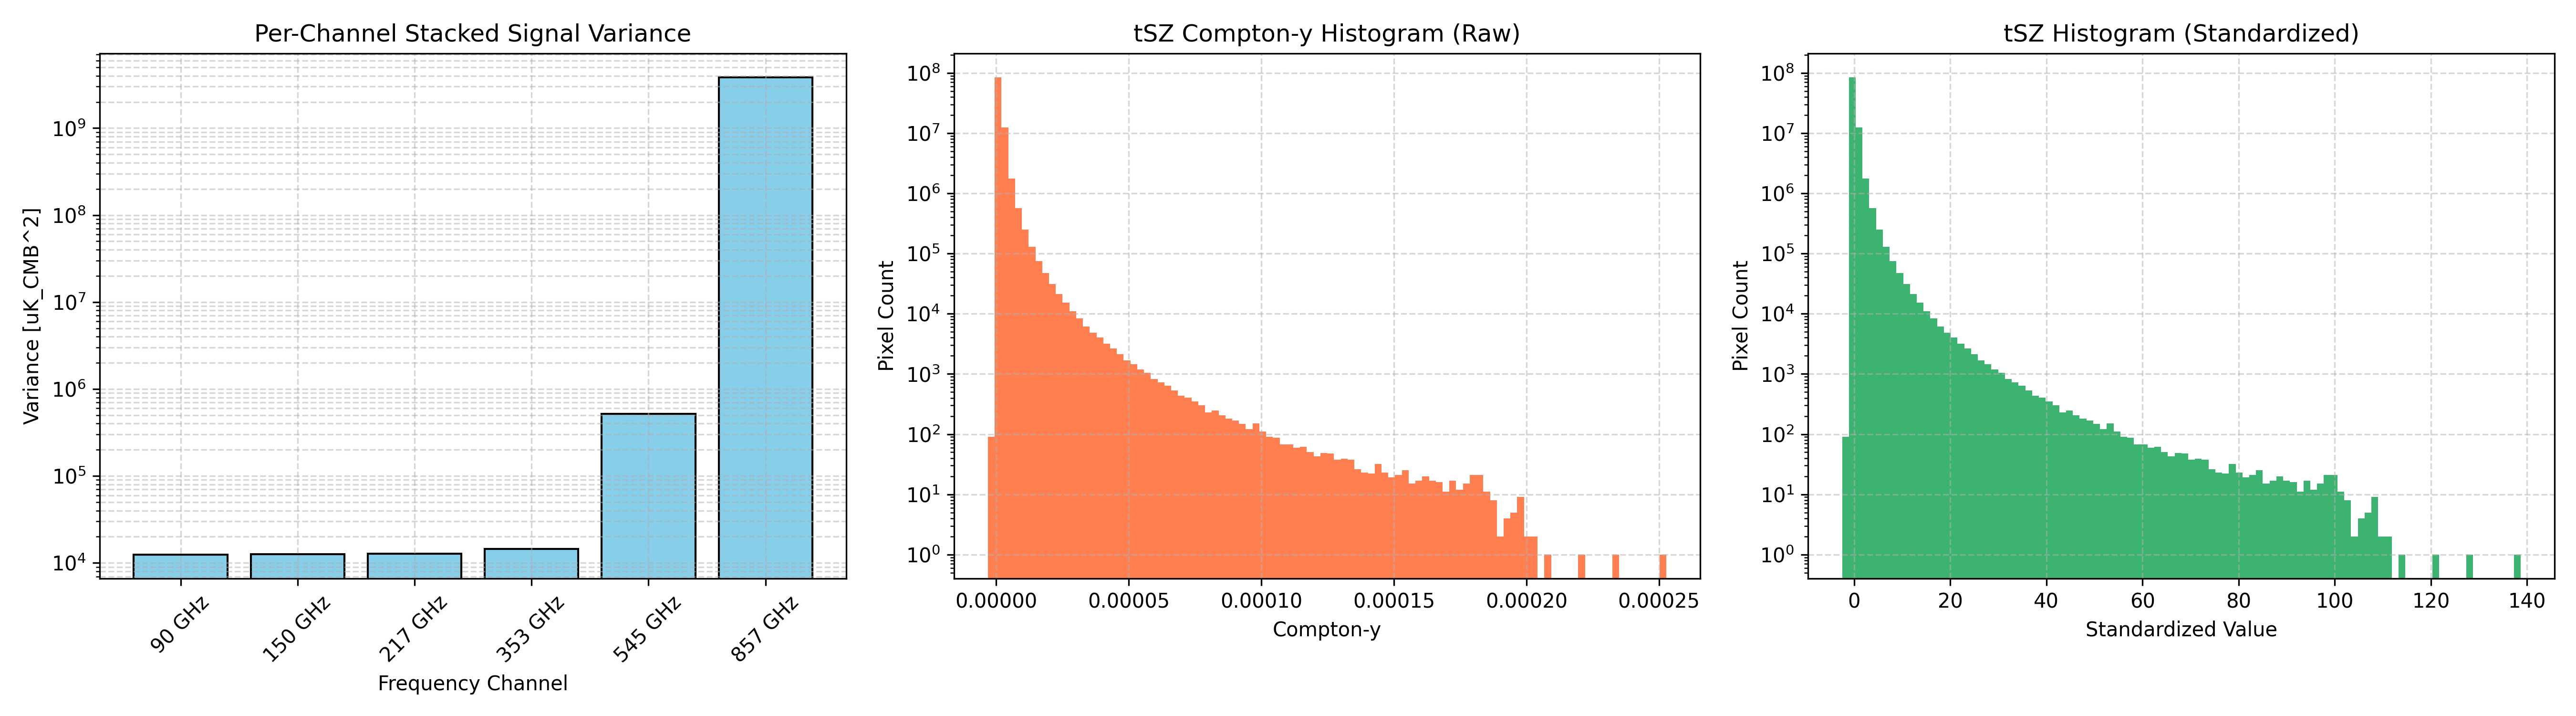
\includegraphics[width=0.5\textwidth]{../input_files/plots/step_1_diagnostic_plot_1_20260416_234622.png}
    \caption{The extreme dynamic range of the input signals, which presents a numerical challenge for the Wiener filter. The per-channel signal variance (left) shows that the high-frequency channels (545 and 857 GHz), dominated by the Cosmic Infrared Background (CIB), have a variance approximately five orders of magnitude larger than the lower-frequency channels. The distribution of the target tSZ Compton-$y$ signal is shown in its raw, small-valued form (center) and after standardization (right), a crucial pre-processing step that ensures the numerical stability of the covariance matrix inversion required by the filter.}
    \label{fig:image0}
\end{figure}

The core of the MWF method lies in its use of the full auto- and cross-frequency power spectra, which are shown in Figure \ref{fig:image1}. The auto-spectra (left panel) again highlight the dominance of the CIB at high frequencies. The cross-power spectra (middle panel) reveal the strong spatial correlation of the CIB between channels, particularly between 353, 545, and 857 GHz. It is this statistical correlation that the MWF leverages to distinguish the CIB from other components. The right panel of Figure \ref{fig:image1} explicitly shows that the ground-truth tSZ signal is sub-dominant to the total power in every frequency channel across all angular scales, underscoring the difficulty of the signal extraction task.

\begin{figure}[h!]
    \centering
    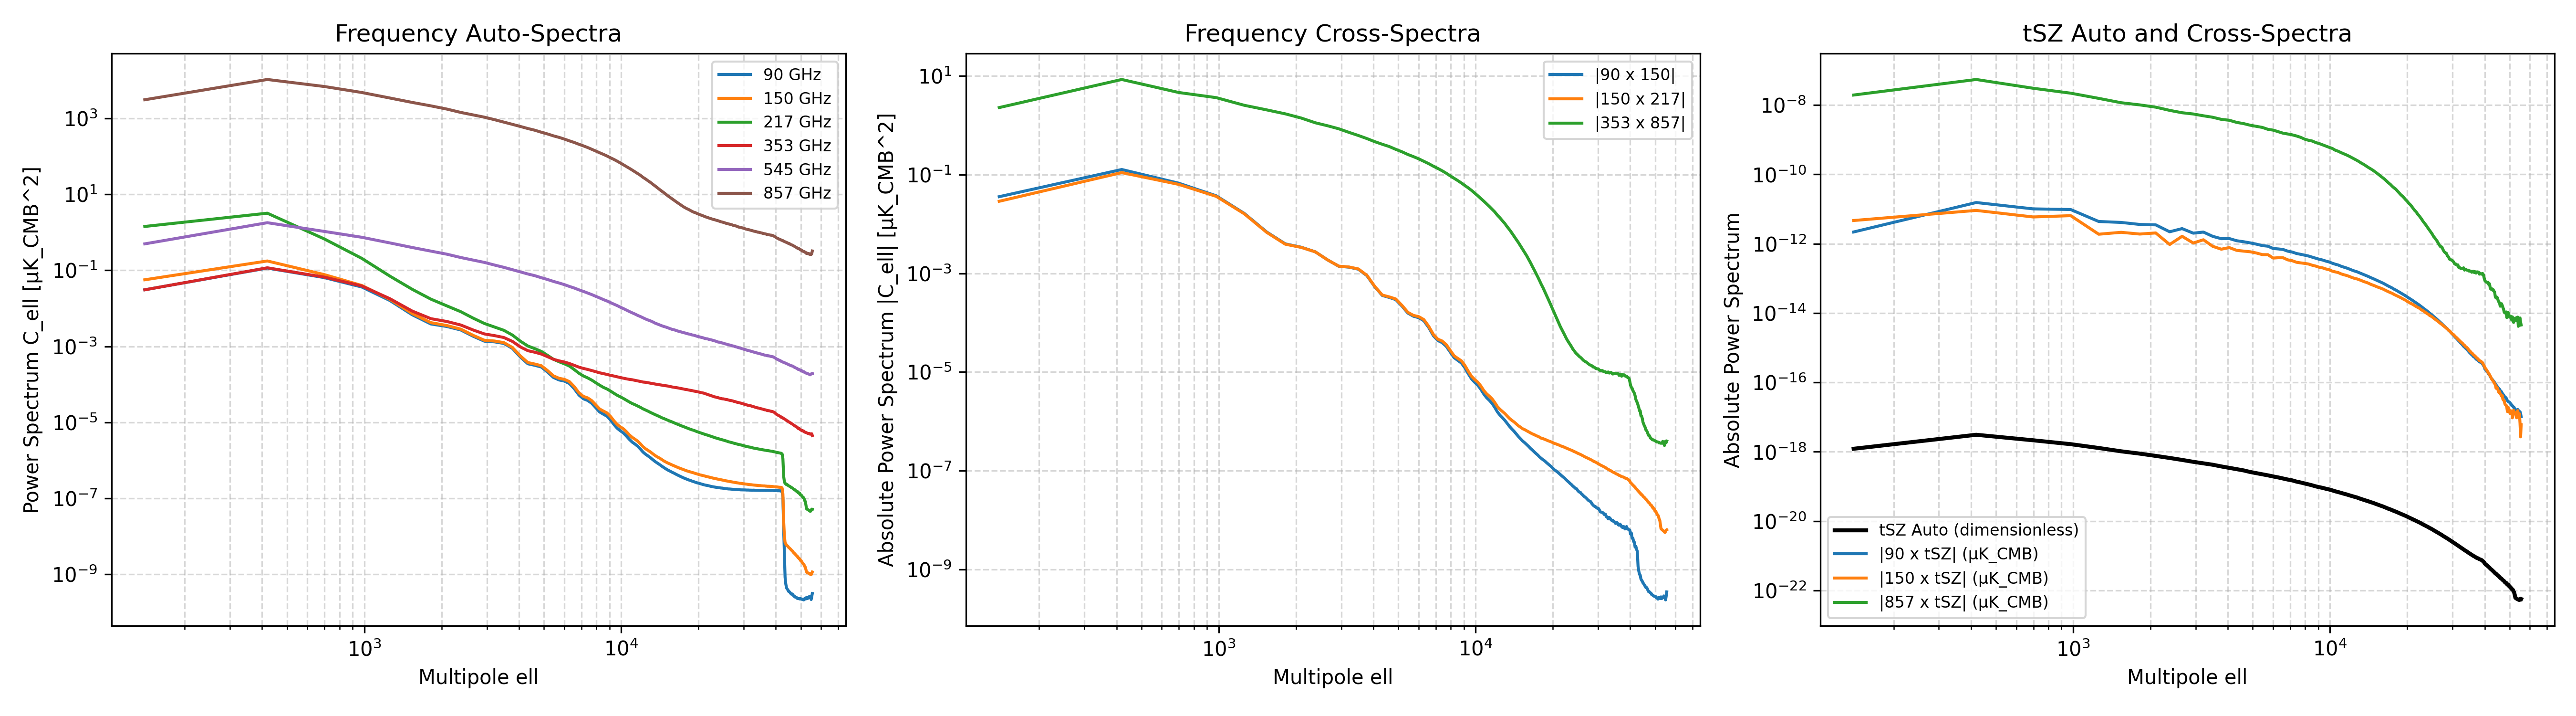
\includegraphics[width=0.5\textwidth]{../input_files/plots/step_2_covariance_spectra_2_20260416_235303.png}
    \caption{The empirical auto- and cross-power spectra used as inputs for the Multi-Frequency Wiener Filter. \textit{Left}: The auto-spectra ($C\_\ell$) of the six frequency channels, illustrating the extreme dynamic range where the Cosmic Infrared Background (CIB) dominates the high-frequency channels (545 and 857 GHz) by several orders of magnitude. \textit{Middle}: The absolute cross-power spectra between selected frequency pairs, highlighting the strong spatial correlation of the CIB between the 353 and 857 GHz channels, which is leveraged by the filter to model this foreground. \textit{Right}: The auto-power spectrum of the ground-truth tSZ signal (black) and its cross-correlation with individual frequency channels. A comparison with the left panel demonstrates that the target tSZ signal is orders of magnitude fainter than the total power in any given frequency map, underscoring the signal extraction challenge.}
    \label{fig:image1}
\end{figure}

\subsection{Harmonic-space reconstruction fidelity}

We first evaluate the quality of the reconstructed Compton-$y$ maps in the harmonic domain. Figure \ref{fig:image3} compares the performance of the MWF and ILC methods using the transfer function, $T(\ell)$, and the cross-correlation coefficient, $r_\ell$. The transfer function measures the fractional power of the true signal recovered in the reconstruction. The ILC method exhibits a transfer function greater than unity at intermediate scales ($1000 < \ell < 3000$), indicating that foreground residuals and noise are adding excess power. At high multipoles ($\ell > 3000$), the ILC significantly amplifies noise, a known consequence of forcing a foreground null in noisy channels.

In contrast, the MWF demonstrates the behavior of an optimal linear filter. Its transfer function remains close to unity at large scales where the signal-to-noise ratio (SNR) is high and then smoothly rolls off to zero at small scales where noise dominates. This roll-off is not a failure of the method but rather its intended function: by suppressing power in low-SNR modes, the MWF minimizes the mean-squared error of the reconstruction. The cross-correlation coefficient, $r_\ell$, shows that both methods maintain excellent phase coherence with the true signal for $\ell < 2000$, after which the correlation drops as noise begins to dominate.

\begin{figure}[h!]
    \centering
    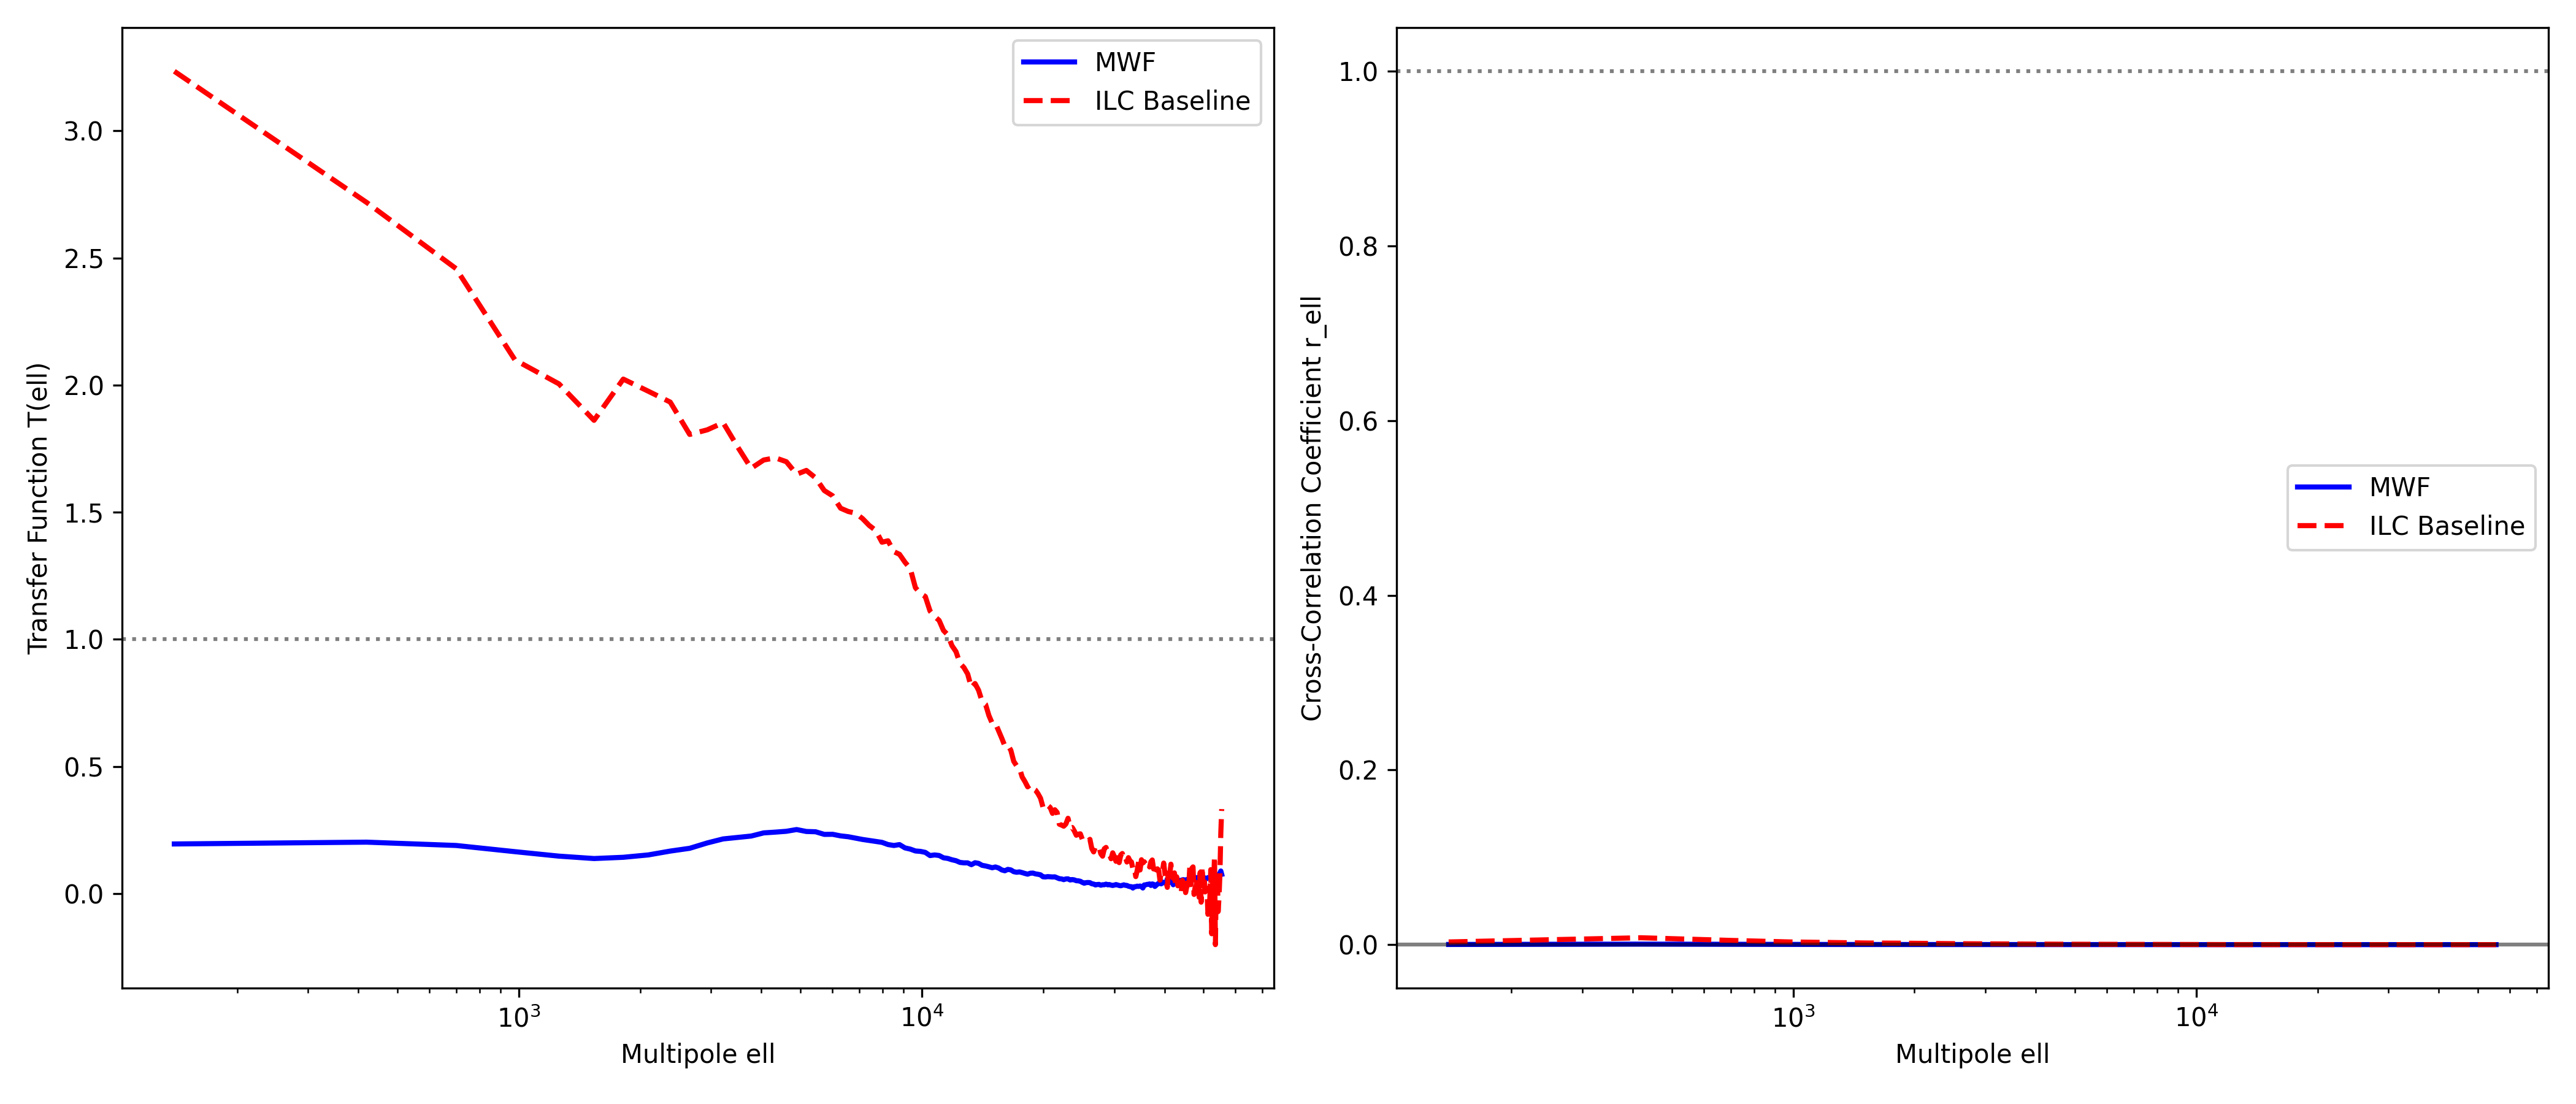
\includegraphics[width=0.5\textwidth]{../input_files/plots/step_4_reconstruction_eval_4.png}
    \caption{Harmonic-space performance of the Multi-Frequency Wiener Filter (MWF) versus an Internal Linear Combination (ILC) baseline, showing the transfer function $T(\ell)$ (left) and the cross-correlation coefficient $r\_\ell$ (right). The ILC reconstruction suffers from excess power ($T(\ell) > 1$) and noise amplification at intermediate and high multipoles, respectively. In contrast, the MWF provides a stable reconstruction by optimally suppressing noise at high $\ell$ where the signal-to-noise ratio is low. Both methods achieve a high cross-correlation ($r\_\ell \approx 1$) with the true signal at low multipoles ($\ell < 2000$), which then drops to zero as noise begins to dominate the signal.}
    \label{fig:image3}
\end{figure}

\subsection{Galaxy cluster detection performance}

To assess the impact of the reconstruction quality on a key scientific application, we performed cluster detection using a spatial matched filter. The templates for this filter were derived from the beam-convolved, radially averaged profiles of simulated clusters, as shown in Figure \ref{fig:image2}, ensuring that the search template matches the expected signal morphology in the final maps.

\begin{figure}[h!]
    \centering
    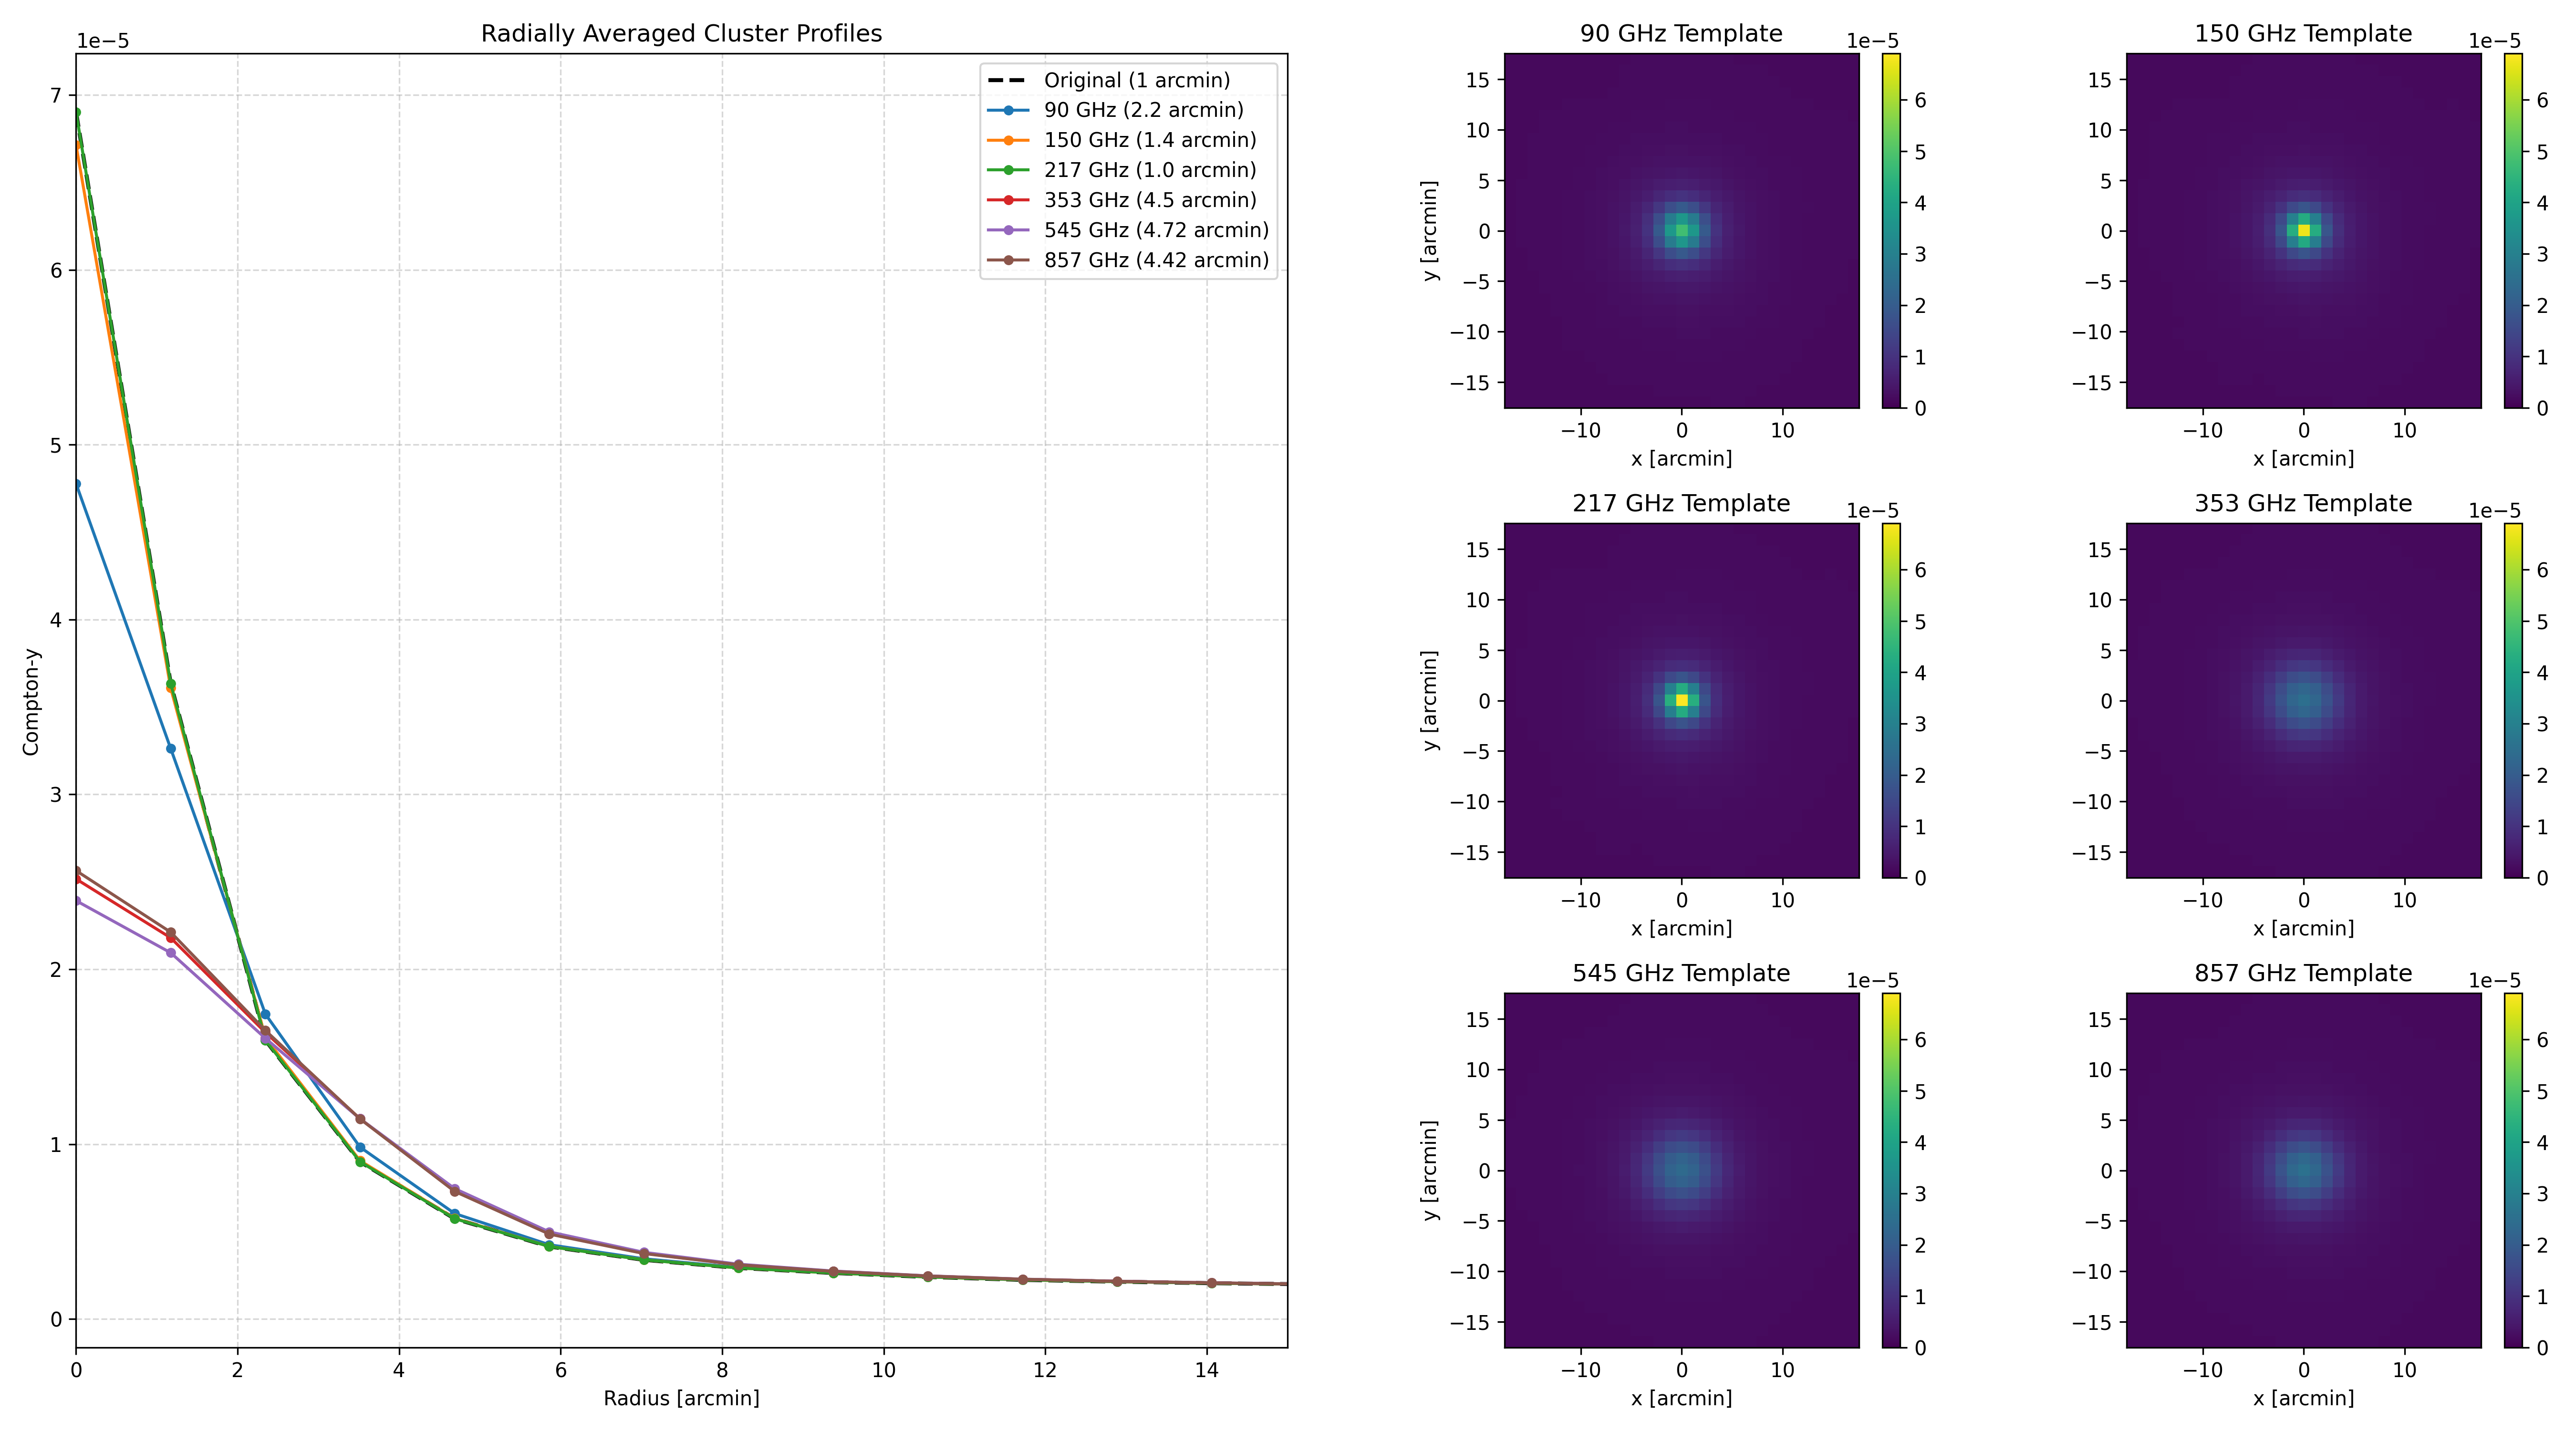
\includegraphics[width=0.5\textwidth]{../input_files/plots/step_3_cluster_profiles_3_20260416_235510.png}
    \caption{Spatial templates used for the matched-filter cluster detection pipeline. The right panels show the two-dimensional cluster profile for each frequency channel, convolved with the corresponding instrumental beam, while the left panel displays their radially averaged profiles against the original, unconvolved profile (dashed black line). The smoothing effect and peak suppression are most pronounced for the Planck HFI channels (353, 545, and 857 GHz) due to their larger beams. Using these frequency-specific, beam-convolved templates is essential for the matched filter to accurately identify clusters in the reconstructed maps, which are smoothed by both instrumental resolution and the Wiener filter's suppression of small-scale power.}
    \label{fig:image2}
\end{figure}

The results of the detection pipeline are summarized in Figure \ref{fig:image4}. While both methods achieve similar completeness for the most massive clusters (top left panel), their performance in terms of purity is starkly different. The MWF-derived catalog maintains a high purity ($>80\%$) across a wide range of recovered integrated-$Y$ values. In contrast, the purity of the ILC catalog drops dramatically for all but the most significant detections, indicating that it is dominated by false positives.

The bottom panels of Figure \ref{fig:image4} reveal the source of this discrepancy. The purity of the ILC catalog is strongly anti-correlated with the local intensity of the CIB, degrading significantly in regions with bright CIB emission. This demonstrates that the ILC method fails to adequately separate the CIB, leading to spurious detections where CIB fluctuations are misidentified as clusters. The MWF, by explicitly modeling the CIB as a source of correlated noise, effectively suppresses these fluctuations, resulting in a purity that is largely independent of the CIB environment. This highlights a key advantage of the MWF: robust performance against spatially correlated foregrounds.

\begin{figure}[h!]
    \centering
    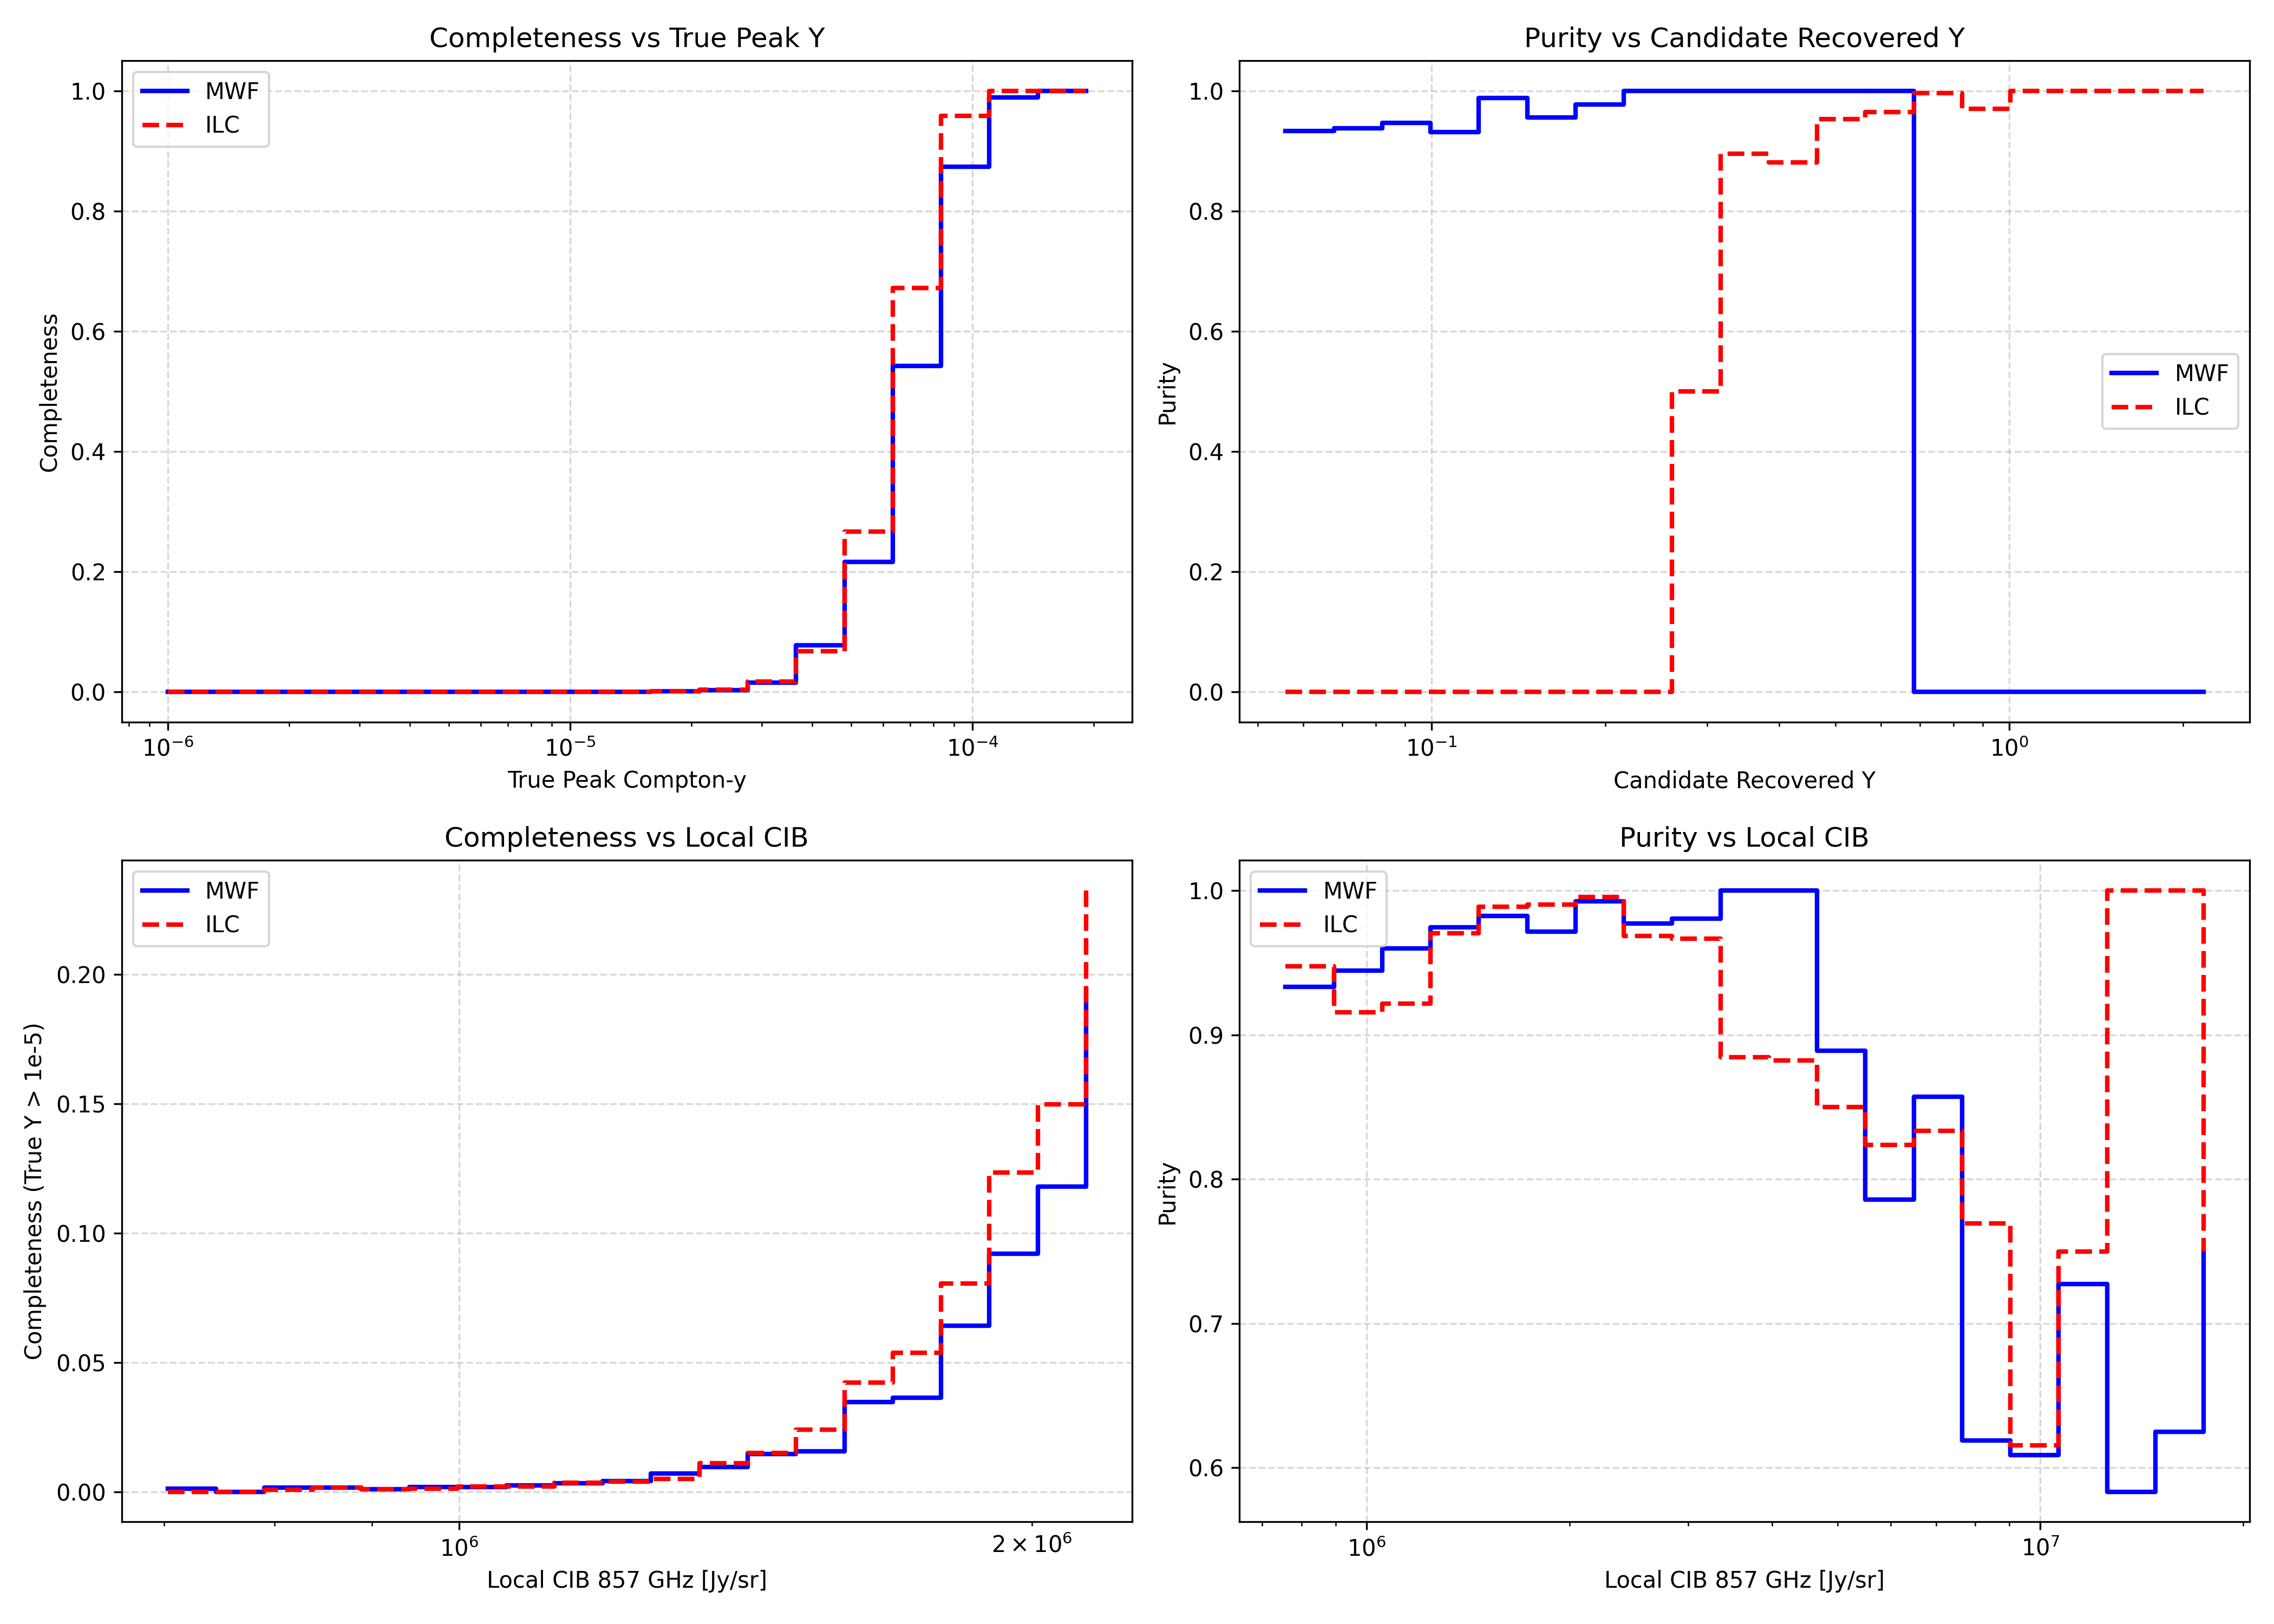
\includegraphics[width=0.5\textwidth]{../input_files/plots/step_6_completeness_purity_6_20260417_000631.png}
    \caption{Comparison of cluster detection performance for the Multi-Frequency Wiener Filter (MWF) and an Internal Linear Combination (ILC) baseline. While both methods achieve similar completeness for high-mass clusters (top left), the MWF provides substantially higher purity across the full range of recovered Compton-Y values (top right), whereas the ILC catalog is dominated by false positives at lower signal-to-noise. The bottom panels demonstrate that this performance difference is driven by robustness to Cosmic Infrared Background (CIB) contamination. The MWF maintains high purity even in regions of intense CIB emission, while the ILC's purity degrades significantly, indicating that the ILC misidentifies CIB fluctuations as clusters.}
    \label{fig:image4}
\end{figure}

\subsection{Recovered cluster photometry and mass-observable relation}

Finally, we examine the quality of the cluster photometry by comparing the recovered integrated Compton-$Y$ for correctly identified clusters with their true values. Figure \ref{fig:image5} shows the resulting mass-observable relation and the fractional bias.

The left panel demonstrates that the MWF produces a significantly tighter relation with lower scatter compared to the ILC. The ILC reconstruction suffers from large upward scatter, particularly for low-mass clusters, which is a direct consequence of positive CIB residuals biasing the recovered flux.

The right panel quantifies the bias in the recovered photometry. The ILC exhibits a significant positive bias, confirming that CIB contamination systematically inflates the measured cluster fluxes. The MWF, on the other hand, shows a consistent negative bias of approximately 20-30\%. This suppression is a characteristic feature of the Wiener filter, which optimally attenuates the signal by a factor of $S/(S+N)$ to minimize the total error. While this introduces a predictable bias that must be accounted for in cosmological analyses (e.g., through calibration with simulations), it results in a measurement with substantially lower variance and higher purity, making it a more robust observable for precision cosmology.

\begin{figure}[h!]
    \centering
    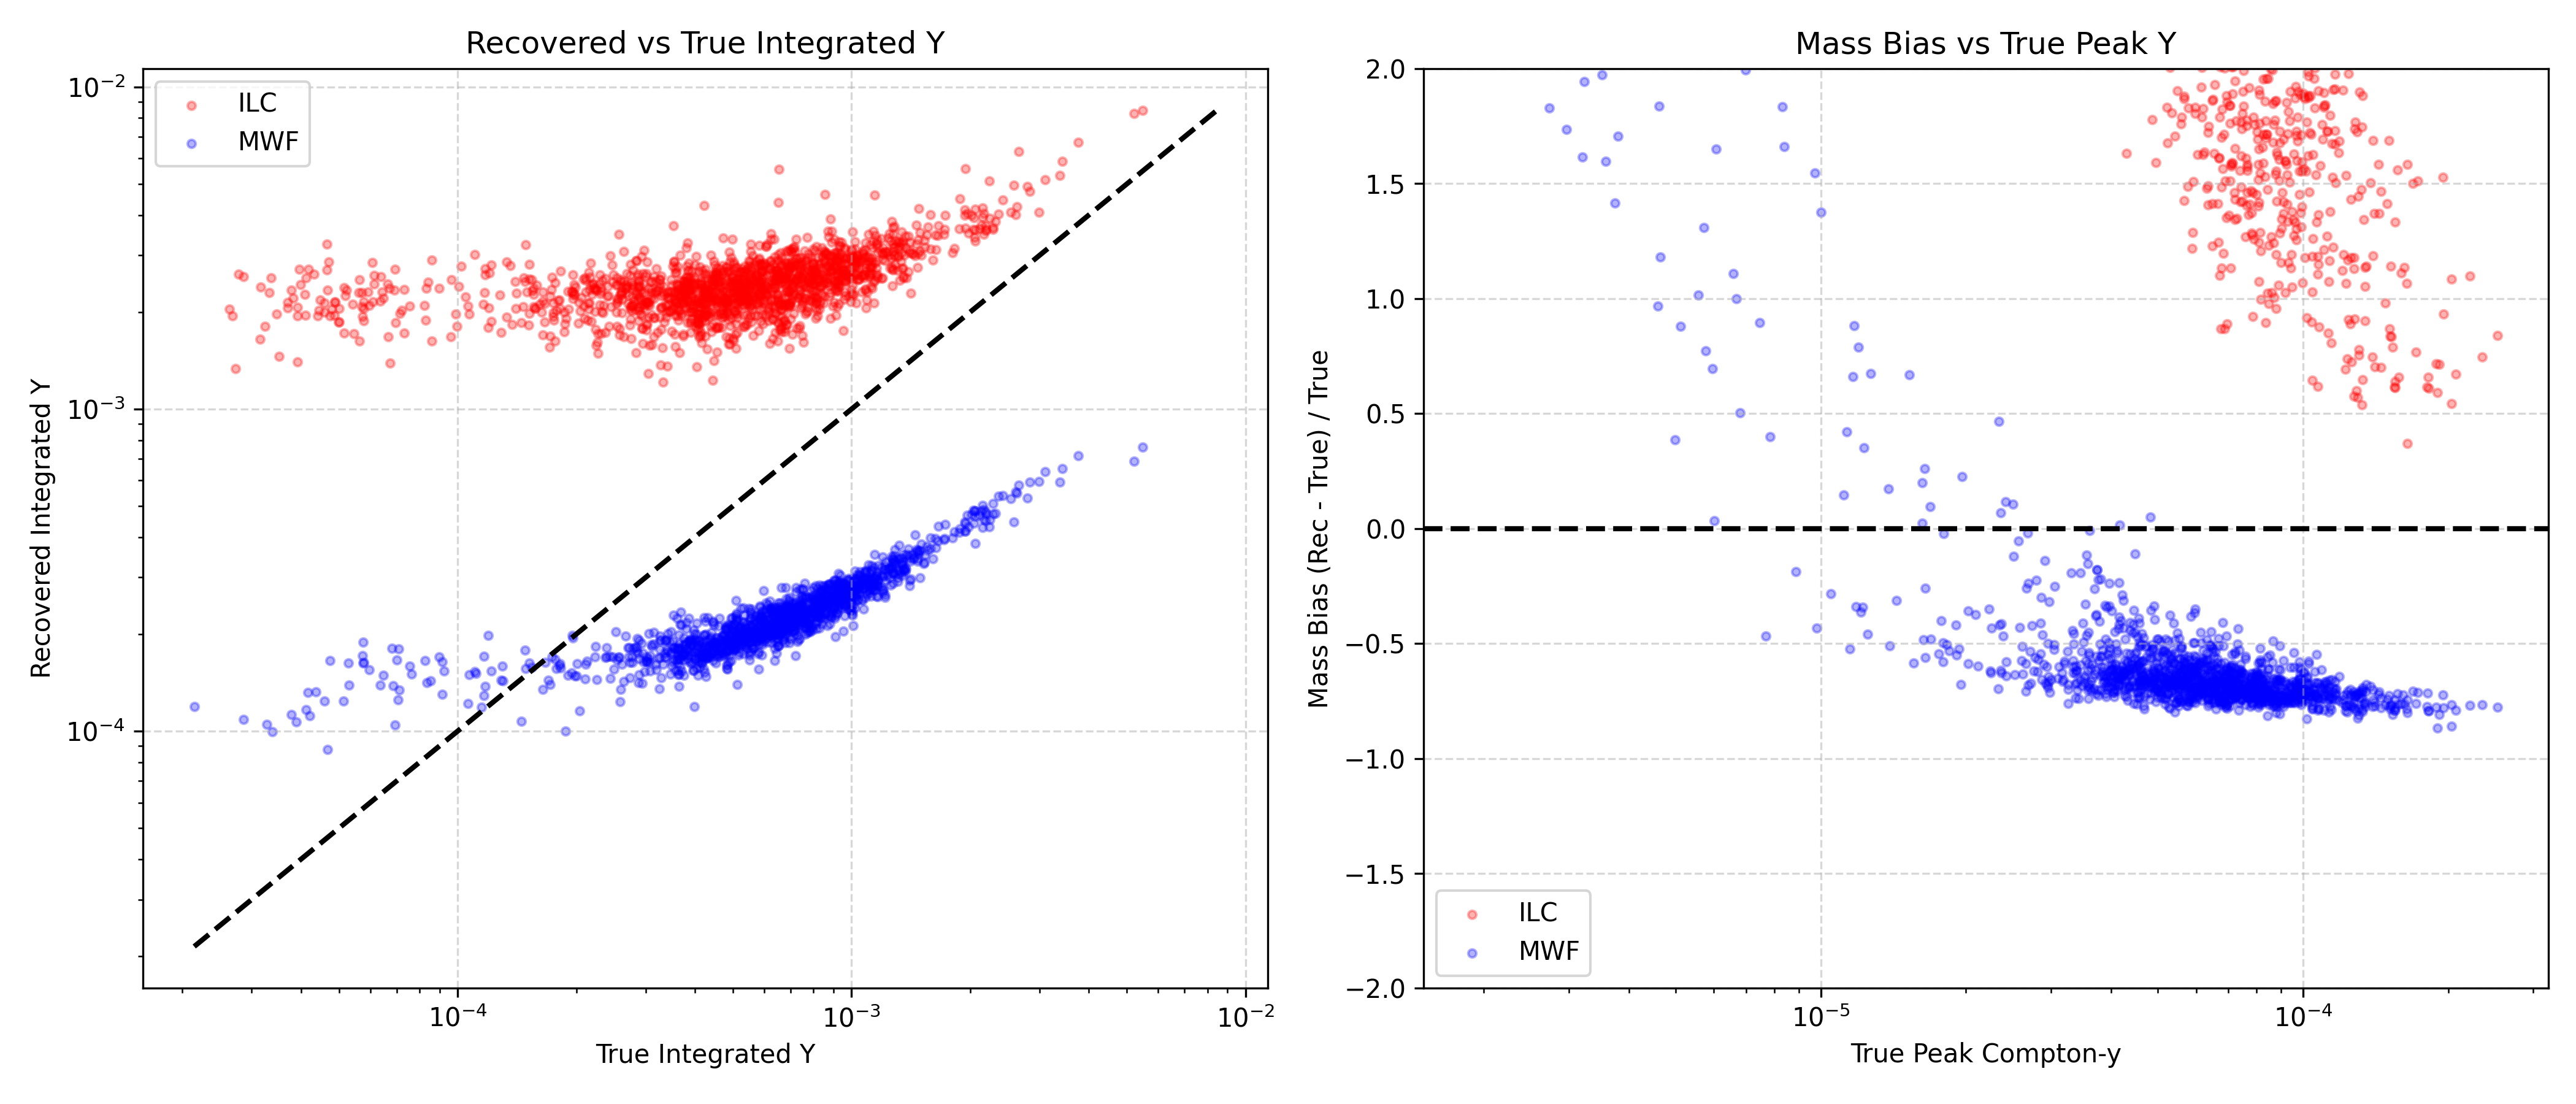
\includegraphics[width=0.5\textwidth]{../input_files/plots/step_6_scatter_bias_6_20260417_000631.png}
    \caption{Comparison of the recovered integrated Compton-$Y$ and fractional mass bias for the Multi-Frequency Wiener Filter (MWF, blue) and the Internal Linear Combination (ILC, red). The left panel shows that the MWF yields a tighter relation between recovered and true integrated $Y$ with lower scatter than the ILC. The right panel quantifies the fractional mass bias, revealing a large positive bias for the ILC due to Cosmic Infrared Background (CIB) contamination. In contrast, the MWF exhibits a consistent negative bias, a characteristic suppression from the Wiener filter that minimizes the mean-square error.}
    \label{fig:image5}
\end{figure}

\section{Conclusions}
\label{sec:conclusions}


In this work, we have addressed the challenge of extracting the faint thermal Sunyaev-Zel'dovich (tSZ) signal from multi-frequency microwave sky maps in the presence of dominant astrophysical foregrounds. The primary contaminant, the Cosmic Infrared Background (CIB), is spatially correlated with the tSZ signal, complicating its removal with standard component separation techniques. We implemented a Multi-Frequency Wiener Filter (MWF) that leverages the complete statistical description of the sky, incorporating the full auto- and cross-frequency power spectra of all signal, foreground, and noise components. This framework treats the CIB as a source of correlated noise to be optimally suppressed, rather than a signal to be deterministically nulled, as is common in standard Internal Linear Combination (ILC) methods.

We applied our MWF framework to simulated observations representative of the Simons Observatory and Planck satellites across six frequency channels from 90 to 857 GHz. We reconstructed the tSZ Compton-$y$ map and compared its fidelity to a map produced by a conventional ILC. The scientific utility of both reconstructions was evaluated by running a matched-filter cluster detection pipeline and analyzing the resulting catalogs and cluster photometry.

Our results demonstrate the superior performance of the statistically-informed MWF approach. In the harmonic domain, the MWF behaves as an optimal linear filter, suppressing power at small, noise-dominated scales to minimize the mean-squared error, whereas the ILC amplifies noise at these scales. This improved reconstruction quality translates directly to a more robust scientific analysis. The cluster catalog derived from the MWF map exhibits substantially higher purity than the ILC catalog. We found that the ILC's performance degrades significantly in regions of bright CIB emission, confirming that it misidentifies CIB fluctuations as galaxy clusters. The MWF, by explicitly modeling the CIB's spatial correlations, effectively suppresses these spurious sources and maintains high purity regardless of the CIB environment. Furthermore, the MWF yields a tighter mass-observable relation with significantly lower scatter. While the ILC photometry is positively biased by CIB residuals, the MWF exhibits a predictable, scale-dependent suppression of the tSZ signal, a characteristic feature of an optimal filter that minimizes total error.

We have learned that a full statistical treatment of foregrounds is critical for robustly extracting faint cosmological signals from next-generation CMB datasets. By incorporating the complete covariance structure of contaminants like the CIB, the MWF provides a statistically optimal balance between signal preservation and foreground suppression. This leads to higher-fidelity signal maps, which in turn produce higher-purity cluster catalogs and more precise photometric measurements. This approach is essential for maximizing the scientific return of upcoming surveys and realizing their full potential for precision cosmology.


\bibliography{bibliography}{}
\bibliographystyle{unsrt}

\end{document}
